\documentclass{article}
\usepackage[T1]{fontenc}

\usepackage{graphicx}
\usepackage{listings}
\begin{document}

\title{FOSS Lab Report}
\author{Gokul K\\[2\baselineskip]
Roll Number: 21\\[2\baselineskip]}
\date{25 January 2020}

\maketitle

\setcounter{section}{3}
\section{Shell Programming I}
\subsection{Aim}
Write shell script to show various system configuration like\newline
   1) Currently logged user and his login name\newline
   2) Your current shell\newline
   3) Your home directory\newline
   4) Your operating system type\newline
   5) Your current path setting\newline
   6) Your current working directory\newline
   7) Number of users currently logged in\newline
\subsection{Source Code}
\begin{verbatim}
#! /bin/bash
clear
log=`who|wc -l`
echo "The current user is $USER"
echo "The current shell is $SHELL"
echo "The home directory is $HOME"
echo "The OS type is $OSTYPE"
echo "the current path setting is $PATH"
echo "The working directory is $PWD"
echo "There are $log users logged in"
\end{verbatim}

\subsection{Output}
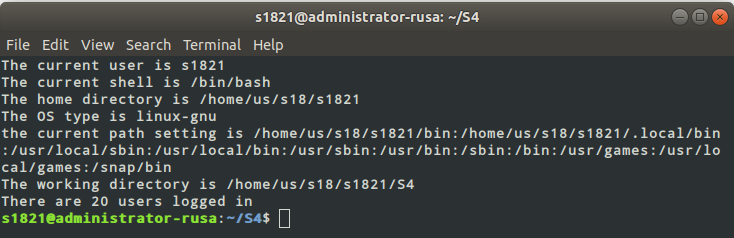
\includegraphics[width=0.8\textwidth]{img/p4.png}

\subsection{Result}
The above program is run on the server shell and the output is recorded.
\end{document}